\documentclass[24pt,b5paper,openright]{book}
\usepackage{packages}

\begin{document}

% Set margins for the title page
\newgeometry{left=2.5cm, right=2.5cm, top=2.5cm, bottom=2.5cm}
% Title page
\begin{titlepage}
    \begin{center}
        \vspace*{1cm}
        \huge{\textbf{Task Priority Control of Underwater Vehicle Manipulator Systems}}
        \vspace{2cm}

        \Large{Håkon Bårsaune}
        \vspace{2cm}

        \large{
            Supervisor: Professor Kristin Ytterstad Pettersen \\
            Co-supervisors: Markus Høgevoll Iversflaten, \\
            Bjørn Kåre Sæbø %TODO: add title?
        }

        \vspace{2cm}
        \today
        \vfill
        \begin{figure}[htbp]
            \centering
            \includesvg[width=0.8\linewidth]{assets/NTNU.svg}
        \end{figure}
    \end{center}
\end{titlepage}

\clearpage
% Restore margins
\restoregeometry 

% Roman numbering for the front matter
\pagenumbering{roman} 

\section*{\Huge{Problem Description}}
\addcontentsline{toc}{chapter}{Problem Description}
The project considers nonlinear control methods for lightweight underwater vehicle-manipulator
systems (light-UVMSs) including both remotely operated vehicles (ROVs) with a lightweight
base, and articulated intervention-AUVs (AIAUVs) (e.g. underwater snake robots) which are
lightweight and with no separate base. Lightweight UVMSs are increasingly taken into use in
several industries, including harbor control and environmental monitoring.

Light-UVMSs reveal a control challenge which has so far has been neglected: to efficiently
control a light-UVMS one should consider the coupling effects between its base and arm
motions. When the arm moves, this will make the base move as well, and vice versa. This
coupling is not so clear for large work-class ROVs where the motion of the heavy base can be
assumed almost decoupled from the motion of the arm. The coupling effects appear partly due
to both reaction forces and hydrostatic forces.

Since UVMSs possess both thrusters and a manipulator arm, these vehicles are considered
kinematically redundant. This makes them very suitable for task-priority control methods. These
methods can be divided into two main groups: velocity- and acceleration-level task-priority
control. Velocity-level control does not explicitly consider all the coupling effects between the
manipulator and the base motions, whereas acceleration-level control does. However, one must
have a sufficiently accurate mathematical model of the UVMS to correctly apply acceleration-
level control. Currently there is a lack of research that compares these methods for underwater
vehicles, especially related to experimental validation.

The task of this assignment is to compare and implement several task-priority control
approaches for light-UVMS and compare their behaviour both theoretically and in simulation.
The main focus should be a comparison between control approaches applied at the velocity and
acceleration levels. The simulation study should be designed to facilitate physical experiments
to validate the findings. NTNU has, through
the AURLab, several vehicles (Eelume, BlueROV, etc.) fit for such experiments.
\newpage
\begin{enumerate}
\item Do a literature survey on task-priority control for underwater vehicle manipulator
systems (UVMS), describe the state-of-the-art, with a focus on works with experimental
results.
\item Write a theoretical comparison of various task-priority methods and their application to
UVMS.
\item Do a simulation study comparing velocity and acceleration level task-priority control
methods for light-UVMS.
\end{enumerate}
The report shall be written in English and edited as a research report including Abstract,
Introduction with motivation, literature survey, contributions of the project work, and the outline
of the report. This is followed by the chapters describing the results of the project work,
simulation results and corresponding discussion, and a conclusion including a proposal for
further work. Source code should be provided in a .zip-file uploaded as an attachment, and with
with code listing enclosed in an appendix in the report. It is supposed that Department of
Engineering Cybernetics, NTNU, can use the results freely in its research work, unless otherwise
agreed upon, by referring to the student’s work.

{
    \color{red}
    Note
    \begin{itemize}
       \item remove the last paragraph?
    \end{itemize}
}

\newpage

\section*{\Huge{Abstract}}
\addcontentsline{toc}{chapter}{Abstract}
Light-UVMS, including 
ROVs and articulated intervention-AUVs, 
are gaining prominence in subsea industries such as harbor control and 
environmental monitoring. These systems present unique control challenges due 
to the strong coupling between base and manipulator arm motions, a phenomenon 
less pronounced in heavier work-class ROVs. This thesis explores task-priority 
control methodologies to address these challenges at both kinematic and dynamic 
levels. A comprehensive simulation framework is developed to facilitate the 
implementation and comparison of these control methods, minimizing the gap 
between simulation and real-world performance. Specifically, kinematic-level 
task-priority control focuses on velocity and acceleration redundancy 
resolution, while dynamic-level control incorporates feedback linearization and 
dynamically consistent inverses to ensure robust task execution 
despite modeling inaccuracies and disturbances. The simulation results 
highlight the strengths  and trade-offs of both control approaches, providing 
insights into their performance, computational efficiency, and robustness under 
varying operational conditions. This work lays a foundation for future 
experimental validation on NTNU’s Eelume 500 articulated intervention-AUV 
advancing the state-of-the-art in underwater robotics.

\newpage

\section*{\Huge{Sammendrag}}
\addcontentsline{toc}{chapter}{Sammendrag}
Lette undervanns-farkostmanipulatorsystem, inkludert fjernstyrt undervanns
farkoster og artikulerte intervensjons-AUV-er, får økende betydning i undervannsindustrien som havneovervåking og miljøovervåking. Disse systemene representerer unike kontrollutfordringer på grunn av den sterke koblingen mellom bevegelser i basen on mainipulatorarmine, et fenomen som er mindre uttalt i tyngere arbeidsklasse-ROV-er. Denne avhandlingen utforsker prioritert oppgavestyring for å håndtere disse utfordringene på både kinematisk og dynamisk nivå. Et omfattende simuleringsrammeverk er utviklet for å muliggjøre implementering og sammenligning av disse kontrollmetodene, og dermed minimere avstanden mellom simulering og ytelse i den virkelige verden.
Kinematisk prioritert oppgavestyring fokuserer på reduntantløsninger for hastinghet og akselerasjon, mens dynamisk kontroll inkluderer tilbakekoblingslinearisering og dynamisk konsistente inverser for å sikre robust oppgaveutførelse til tross for modellfeil og forstyrrelser. Simuleringsresultatene fremhever styrkene og avveiningene ved begge kontrolltilnærmingene, og gir innsikt i deres ytelse, beregningsmessige effektivitet og robusthet under varierende operasjonelle forhold. Dette arbeidet legger grunnlaget for fremtidig eksperimentell validering på NTNU's Eelume 500 artikulerte intervensjons-AUV, og fremmer utvikling innen undervannsrobotikk.

\newpage

\section*{\Huge{Preface}}
\addcontentsline{toc}{chapter}{Preface}
I would like to express my gratitude to my co-supervisors, Markus H.
Iversflaten and Bjørn K. Sæbø, for their guidance and support throughout this
project. Their support in selecting relevant literature, providing detailed
feedback on my written work, and offering direction at critical stages has been
essential to the progress and completion of this thesis.

Additionally, I extend my thanks to my good friend, Tor Børve Rasmussen,
for his thoughtful discussions and constructive feedback regarding the content
of the thesis and the quality of the code.


\DTMlangsetup{showdayofmonth=false}
\begin{flushright}
    \textit{Håkon Bårsaune} \\
    \textit{Trondheim,\today}
\end{flushright}
\DTMlangsetup{showdayofmonth=true}
\newpage

\tableofcontents
\newpage

% List of figures and tables, they don't need take two pages each
\begingroup
\let\cleardoublepage\relax
\let\clearpage\relax
\listoffigures
\newpage
\listoftables
\endgroup


\chapter{Introduction}
\pagenumbering{arabic} % Arabic numbering for the main matter
% Change the page style to include the chapter number and title in the header
\fancyhead[RE]{\thepage}
\fancyhead[LE]{\MakeUppercase{\rightmark}}
\fancyhead[LO]{\thepage}
\fancyhead[RO]{\MakeUppercase{\leftmark}}
\fancyfoot[C]{}

This chapter introduces the core motivation behind the thesis and outlines the
context and importance of the work. The driving factors and key challenges that
led to the thesis are presented. A brief overview of the literature that is
relevant to the thesis is given, and the assumptions made are
stated. The chapter concludes with a summary of the contributions of this thesis,
as well as an outline of the subsequent chapters.


% ------------------------------------------------------------------ Motivation
\section{Motivation}

{
    \color{red}
    \begin{itemize}
        \item Highly redundant systems $\rightarrow$ Task-priority control
        \item Inaccurate models? How good is TPC for light-UVMS?
            \begin{itemize}
                \item Kinetic vs Dynamic redundancy resolution
            \end{itemize}
        \item Need for realistic simulations and dynamic models when comparing TPC methods
    \end{itemize}
}

In 2015, the United Nations adopted the 2030 Agenda for Sustainable Development
\cite{UN2030Agenda}, which outlines 17 Sustainable Development Goals (SDGs) to
address global challenges such as poverty, inequality, climate change, and
environmental degradation. The research and methods presented in this thesis
contribute to the achievement of several of these goals. For example, \emph{SDG 14
Life Below Water}, "Conserve and sustainably use the oceans, seas and marine
resources for sustainable development.". UVMSs can monitor and inspect underwater
infrastructure, reducing the risk associated with oil spills, structural failures,
or leaks. Furthermore, UVMSs controlled in a task-priority manner can perform automated
high resolution imagery and data collection, identifying and mitigating potential
damage and disruptions to marine ecosystems.

\emph{SDG 9 Industry, Innovation, and Infrastructure} aims to "Build resilient
infrastructure, promote inclusive and sustainable industrialization and foster
innovation. This can be achieved by enhancing underwater infrastructure reliability
through regular and automated inspection and maintenance, reducing the risk of
structural failures and environmental damage. This thesis also promotes innovation
in the field of maritime robotics, leading to more advanced technologies for
sustainable ocean management.

Finally, \emph{SDG 13 Climate Action} aims to "Take urgent action to combat climate
change and its impacts". UVMSs can facilitate oceanographic research by collecting
environmental data and monitoring climate change, laying the groundwork for actions
to combat the effects of climate change. UVMSs can support the development of
sustainable marine energy solutions, such as offshore wind farms and wave energy.

In summary, by aligning with key SDGs, this research demonstrates the potential
for sustainable innovation in underwater systems, contributing to a resilient 
and environmentally conscious future.

% ------------------------------------------------------------ Literature Review
\newpage
\section{Literature Review}

Some of the earliest works on task-priority control were introduced in 
\cite{hanafusa1981}. This study proposed a method for controlling redundant 
manipulators through a task-priority control scheme, enabling the simultaneous 
execution of two tasks. Specifically, the framework was applied to a 7-DOF 
manipulator tasked with tracking a desired end-effector position while 
maintaining a constant arm posture. This approach was later expanded in 
\cite{nakamura1987}, where a more comprehensive formulation was presented, 
along with the introduction of potential functions for obstacle avoidance.

Building on the foundations laid by \cite{hanafusa1981}, \cite{nakamura1987}, 
and others, the work in \cite{siciliano1991} extended the task-priority 
framework to accommodate an arbitrary number of tasks. The proposed formulation 
employs a recursive approach, enabling efficient computation of joint 
velocities. A simulation study demonstrated the method's effectiveness in 
controlling a 7-DOF planar manipulator performing three tasks, including 
obstacle avoidance. The challenges posed by algorithmic and kinematic 
singularities were later addressed in \cite{chiaverini1997}. While kinematic 
singularities can lead to excessively large joint velocities, algorithmic 
singularities may cause strict task priority to break down. To mitigate these 
issues, the study introduced damped pseudo-inverse matrices as a solution.

One notable limitation of the frameworks discussed so far is their assumption 
of decoupled kinematics and dynamics. However, in real-world 
systems—particularly in underwater vehicle-manipulator systems (UVMSs)—this 
assumption does not hold. To address this limitation, \cite{khatib1987} 
proposed a framework for redundancy resolution at the dynamic level. This 
approach incorporates task dynamics, employs feedback linearization techniques, 
and utilizes dynamically consistent generalized inverses \cite{khatib1995} to 
maintain strict task priority. However, this method relies heavily on an 
accurate dynamic model, which can be a tradeoff for addressing coupled dynamics 
and kinematics. The framework was further extended in \cite{khatib2004,sentis2004}, 
allowing it to handle an arbitrary number of tasks effectively. In this work, a 
high-DOF humanoid robot was successfully controlled in a simulation study.

Stability analysis of kinematic-level priority-based control schemes for 
redundant manipulators was conducted in \cite{antonelli2009}. Using a 
Lyapunov-based approach, the study provided sufficient conditions for stability 
based on control gains and task design. However, the proposed method assumes 
decoupled kinematics and dynamics, making it less directly applicable to UVMSs 
without additional assumptions regarding the relative speeds of robot dynamics 
and inverse kinematics.

A task-priority control scheme specifically applied to UVMSs was presented in 
\cite{antonelli1998}. This work employed a kinematic-level task-priority 
control approach to control a 6-DOF articulated underwater vehicle (AUV) 
equipped with a 3-DOF planar manipulator arm. While the simulation results were 
promising, the study did not account for the system's dynamics.

In recent years, approaches that incorporate dynamic considerations have been 
developed. For example, \cite{basso2020} introduced a method that uses control 
Lyapunov function-based quadratic programming to address control allocation, 
dynamic control, and redundancy resolution in redundant robotic systems. Given 
the challenges posed by disturbances and modeling inaccuracies in UVMS 
dynamics, \cite{iversflaten2022} proposed a dynamic controller based on sliding 
mode control. A simulation study demonstrated the effectiveness of this method 
in handling these challenges. Regarding physical experiments on UVMSs, there 
seem to be a lack of research that compares the performance of the proposed 
task-priority control methods in a real-world setting.



% Might want to include some articles on vehicle modeling?

% ----------------------------------------------------------------- Assumptions
\section{Assumptions}
\begin{enumerate}
    \item \emph{Assumption 1}
    \item \emph{Assumption 2}
    \item \emph{Assumption 3}
\end{enumerate}

% --------------------------------------------------------------- Contributions
\section{Contributions}

The main contributions as presented in this thesis are as follows:
\begin{itemize}
    \item \emph{A Python library for generating dynamic models of UVMSs, allowing
        for rapid prototyping of models.}
    \item \emph{A simulator in C++, together with a set of task-priority controllers
        ,using the generated models to simulate the behavior of UVMSs.}
    \item \emph{A simulation study comparing velocity and acceleration level
        task-priority control methods for light-UVMS.}
\end{itemize}

% -------------------------------------------------------------- Thesis Outline
\section{Thesis Outline}

\emph{Chapter 2} gives an overview of the background and preliminaries of the
thesis. The chapter introduces the mathematical tools and concepts used throughout
the thesis. \emph{Chapter 3} presents the mathematical modelling of underwater
vehicle manipulator systems (UVMs). \emph{Chapter 4} introduces the Python library
\pymuvs and explains how it can be used to model underwater vehicles. \emph{Chapter 5}
presents the simulation study comparing velocity and acceleration level task-priority
control methods for light-UVMS. \emph{Chapter 6} concludes the thesis and outlines
possible future work.

\chapter{Background and Preliminaries}

\chapter{Modelling}

\chapter{PyMUVs}
\emph{\textbf{Py}MUVs \textbf{M}odels \textbf{U}nderwater \textbf{V}ehicle\textbf{s}}

% -----------------------------------------------------------------------------
\section{Introduction}

\pymuvs{ }is a Python library for mathematically modelling underwater vehicles. The
library is designed to be modular and easy to use, and is built on top of NumPy
\cite{numpy} and SymPy \cite{sympy}. By defining the a set of links, as well as
their properties, such as mass, inertia, volume, linear drag, quadratic drag,
external forces, and transformations between links,
\pymuvs{ }can compute a symbolic representation of the system on the
form
\begin{align}
    \bm{M}(\bm{q}) \ddot{\bm{q}} + \bm{C}(\bm{q}, \dot{\bm{q}}) \dot{\bm{q}} +
    \bm{D}(\bm{q}, \dot{\bm{q}}) \dot{\bm{q}} + \bm{g}(\bm{q}) = \bm{J}^T(\bm{q}) \bm{B} \bm{u},
    \label{eq:pymuvs:eom}
\end{align}
where the matrices $\bm{M}$, $\bm{C}$, $\bm{D}$, $\bm{g}$, $\bm{J}$, and $\bm{B}$ are
computed symbolically and can be used to simulate the system. This is especially
useful when implementing model-based controllers that require the dynamics of the
system to be on the form of, or similar to \autoref{eq:pymuvs:eom}. The library
also supports exporting the symbolic representation, and the whole model to C++
code, which can be used in real-time simulations or for significantly faster
simulations.
The library, written in Python, allows for quick and easy prototyping of
models, with the flexibility to add or remove links and transformations.
The library is open-source and can be found at
\url{https://github.com/haakonbaa/pymuvs}. 


% -----------------------------------------------------------------------------
\subsection{Motivation and Importance}

\begin{itemize}
\item Why pymuvs was created
    \begin{itemize}
    \item Gazebo can be used to simulate underwater vehicles, but it does not provide
    the model matrices needed for model-based control.
    \item Existing simulators existed, but they were either written in Rust, which
    is not as widely used as Python, or they were not as flexible as we wanted.
    \end{itemize}
\item Features
\item Assumptions
\item C++ code generation
\item The goal is to develop a controller on the eelume robot, this needs to be fast
which facilitates the development of controllers in a microcontroller environment
as well as puts restrictions
\end{itemize}

% -----------------------------------------------------------------------------
\section{Architectural Design}

\subsection{Overall Structure}

\subsection{Core Modules}

\subsection{Dependencies}

% -----------------------------------------------------------------------------
\section{Implementation details}

\subsection{Model Definition}

\subsection{Customization}

\subsection{Validation and Testing}

% -----------------------------------------------------------------------------
\section{User Guide}
\subsection{Installation}

% -----------------------------------------------------------------------------
\section{Simulator}

In addition to the \pymuvs{} library, a dedicated simulator was developed to 
model the dynamics of various underwater vehicles. The simulation results 
presented in this thesis are derived from models created using \pymuvs{}, with 
corresponding C++ code generated from these models. A custom C++ implementation 
was developed to utilize the \pymuvs{}-generated code for simulating the 
system. Throughout this thesis, this implementation is referred to as 
\textit{the simulator}.

The simulator employs the fourth-order fixed-step Runge-Kutta method, as 
described in \autoref{sec:runge-kutta}, to integrate the system dynamics. This 
method was selected due to its simplicity and reliable performance. 
Implementing the simulator in C++ offers several advantages. Firstly, C++ 
provides a highly efficient simulation environment, which is particularly 
valuable during controller design and parameter tuning. Additionally, 
controllers can be implemented directly in C++ and executed within the same 
simulation environment, an essential feature for real-time controller development.

The simulator also facilitates seamless integration with higher-level 
programming languages such as MATLAB or Python. Through C++ wrappers, 
controllers implemented in these languages can be executed alongside the 
simulation. Similarly, low-level programming languages like Rust, Go, or C can 
be compiled into shared libraries and dynamically linked with the C++ 
simulator, enabling flexible integration across different software ecosystems.

One significant benefit of using C++ is the ability to perform simulations 
faster than real-time. To demonstrate the simulator's performance, a benchmark 
test was conducted with the following parameters: a simulation time of $100 \, 
\mathrm{s}$, a time step of $\Delta t = 0.01$, and a simple PD-controller. The 
simulator successfully simulated a 3-link system with 10 states in an average 
time of $0.3757 \, \mathrm{s}$, with a standard deviation of $3.4908 \, 
\mathrm{ms}$, across 10 runs. This corresponds to a speedup factor of 
approximately $266$ times faster than real-time.

It is important to note that the mass matrix in \autoref{eq:pymuvs:eom} must be 
inverted four times per time step when evaluating $\ddot{\bm{q}}$. While the 
simulation's performance may vary based on factors such as controller 
complexity, model intricacy, and computational hardware, it is evident that the 
simulator offers a highly efficient and robust environment for dynamic system 
simulations.

% -----------------------------------------------------------------------------
\section{Conclusion}

\iffalse

\section{Modules}
The following sections will give an overview of the modules making up the
library as well as some brief examples showing basic use cases. Note that this
is not a complete overview of the library, but rather a brief introduction to
the most important functionality of each module.

% ------------------------------------------------------------------------- se3
\subsection{se3}
The \texttt{se3} module contains functions for working with the special Euclidean
group $SE(3)$. The module is built on top of \texttt{SymPy} and provides functions for
generating elements of $SE(3)$ from \texttt{SymPy} symbols, as well as functions
for computing the inverse and multiplication of the elements. A simple example
is shown below.

\begin{figure}[h]
    \centering
    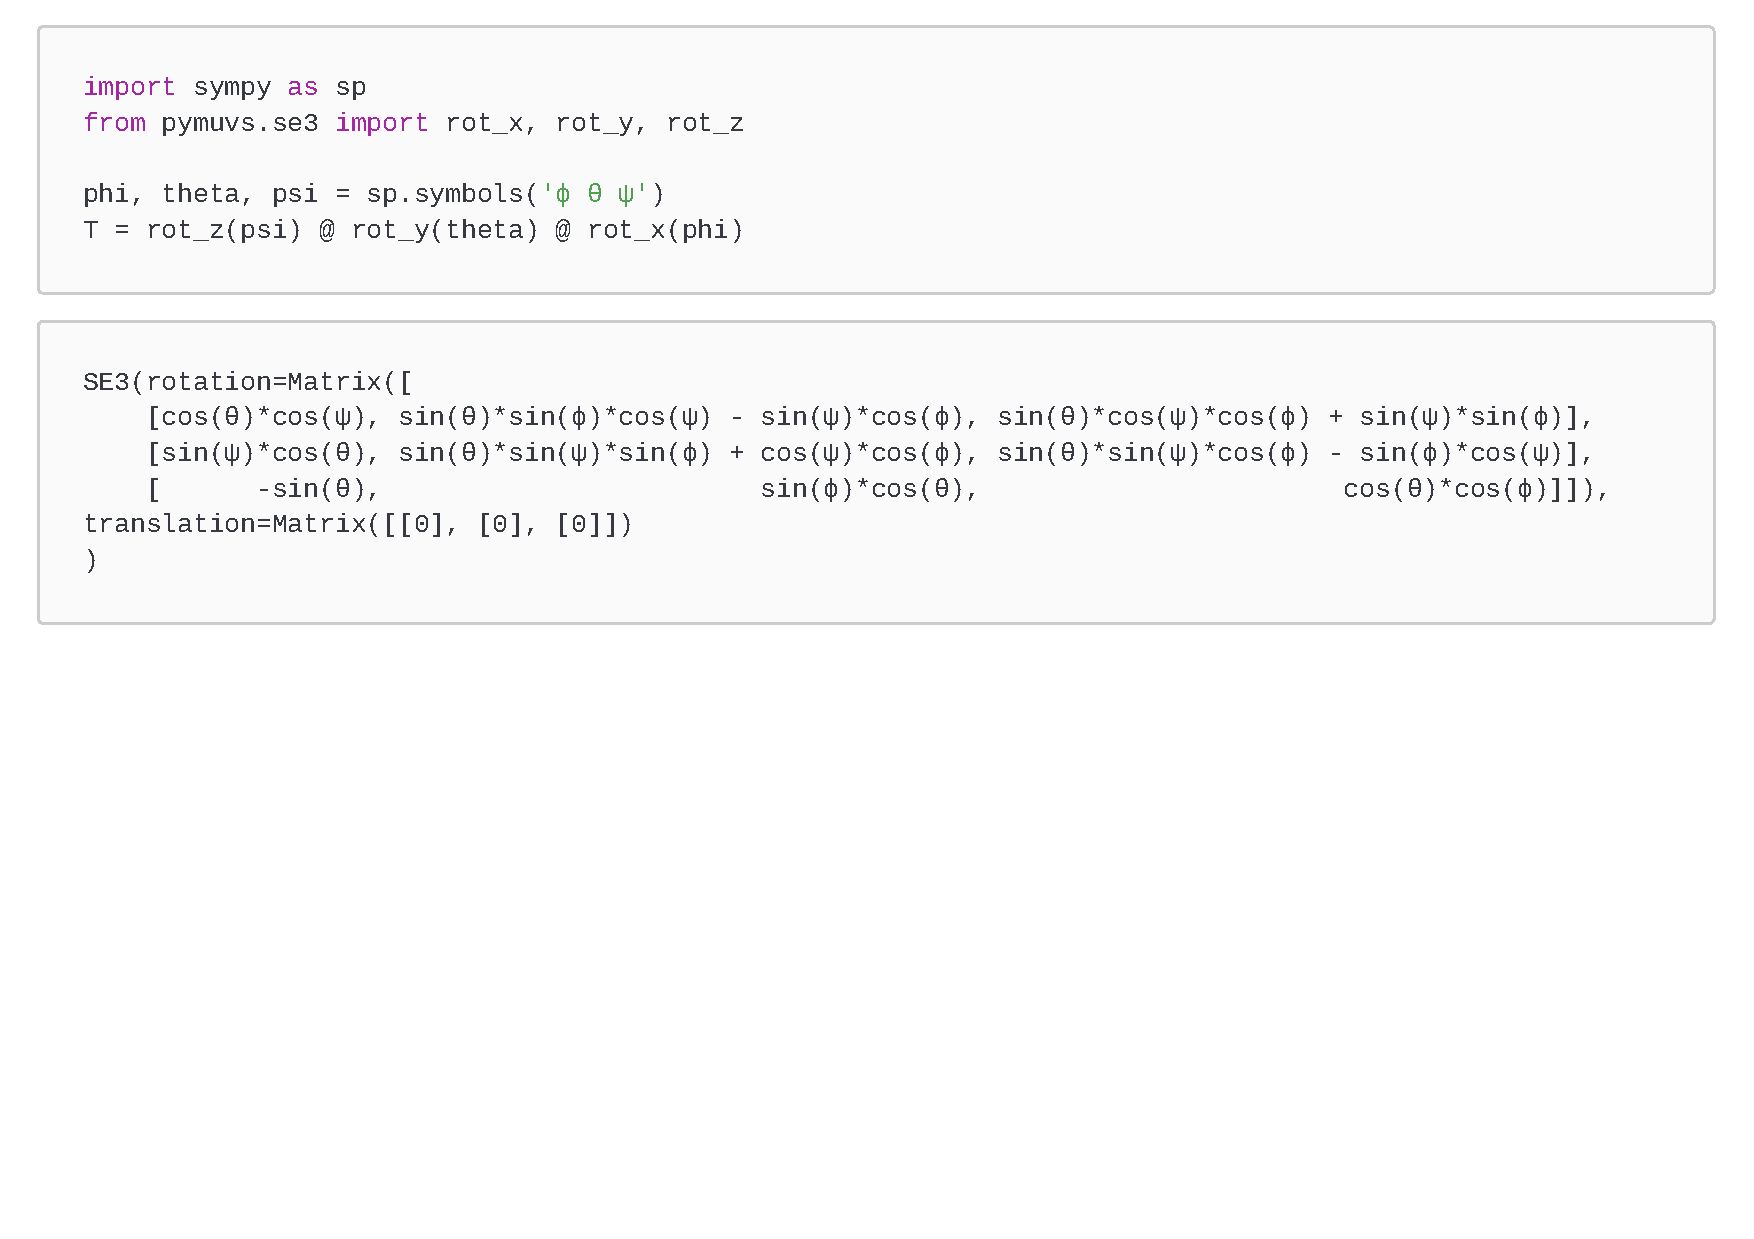
\includegraphics[page=1,width=\linewidth,trim=0 11cm 0 0]{assets/se3.pdf}
    \caption{Example usage of the \texttt{se3} module.}
    \label{fig:usage:se3}
\end{figure}

\autoref{fig:usage:se3} shows how to create a variable $T \in \SO$ representing
a pure rotation in euler angles. More elements of this class can be composed
together to form arbitrary transformations. This group is used in other modules
to represent the transformations between links in a robot model.

% --------------------------------------------------------------------- util
\subsection{util}


% --------------------------------------------------------------------- codegen
\subsection{codegen}
The \texttt{codegen} module is used to generate C++ code from a model. The module
uses the \texttt{sympy.ccode} function to generate C code from
each expression in every matrix and combines them into a header and a source
file. The \texttt{Eigen} library \cite{eigen3} is used to represent the matrices.

\begin{figure}[h]
    \centering
    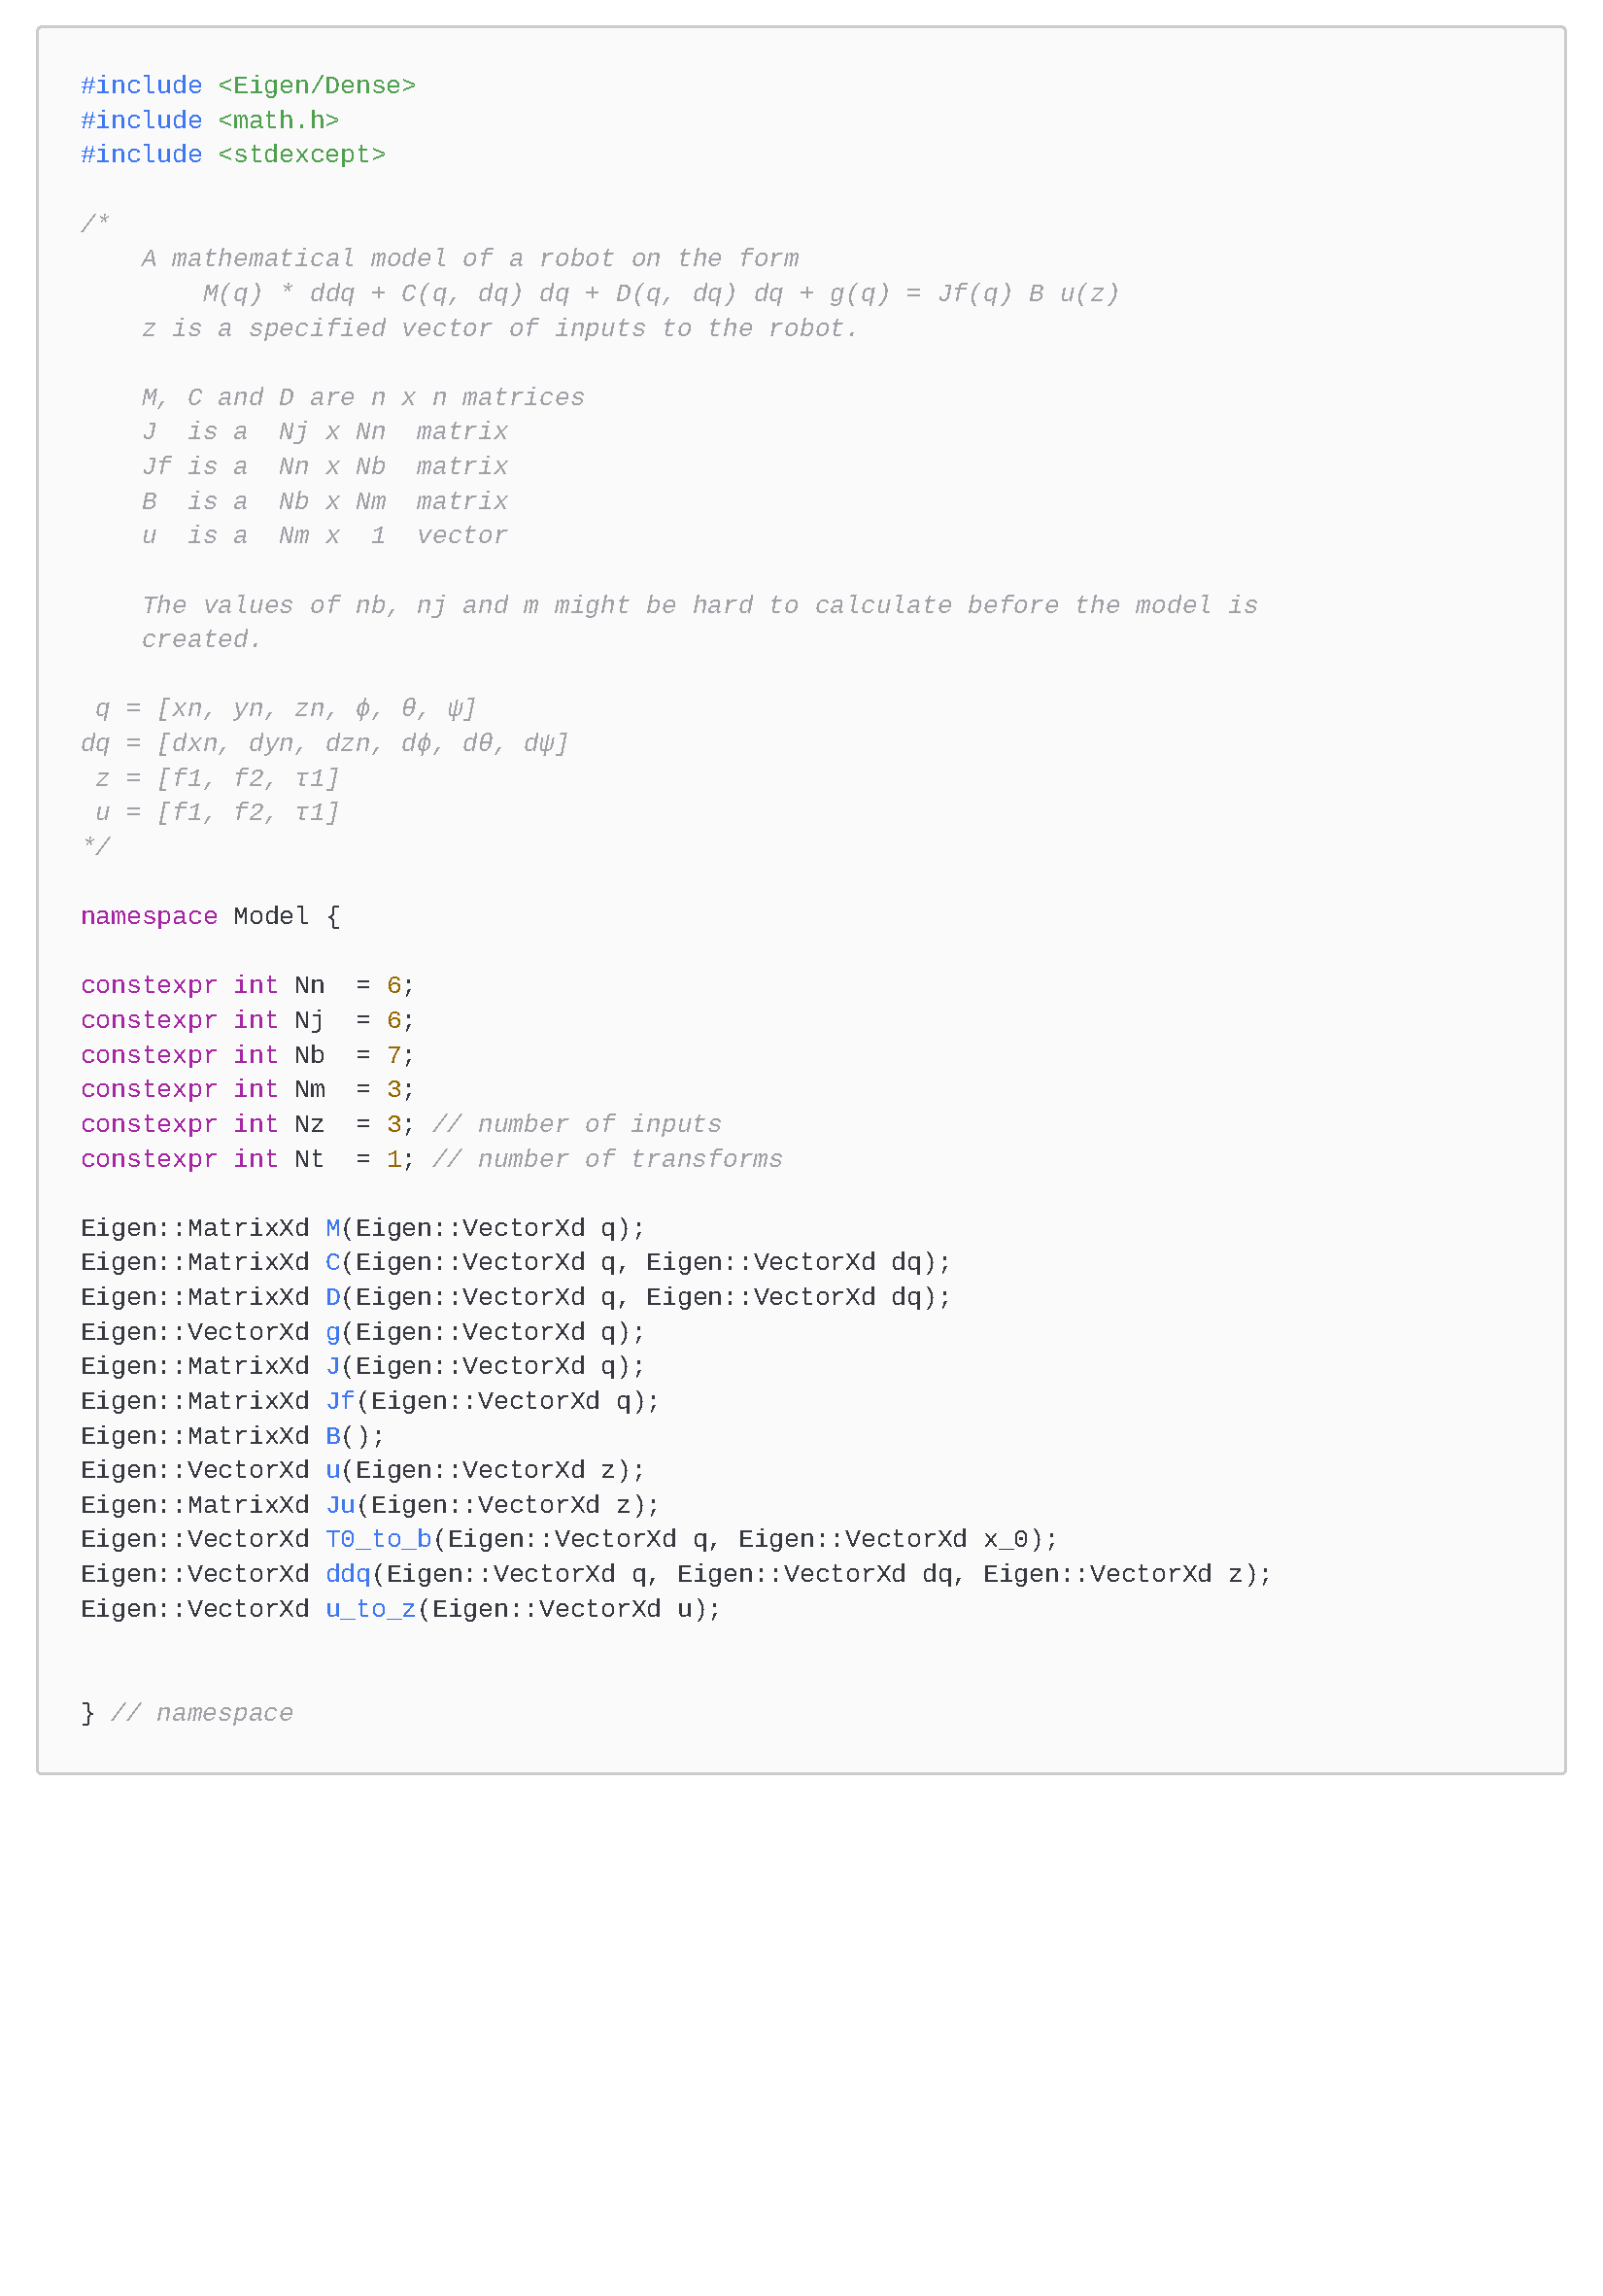
\includegraphics[page=1,width=\linewidth,trim=0 9cm 0 0]{assets/codegen.pdf}
    \caption{Automatically generated c++ code from a model.}
    \label{fig:codegen}
\end{figure}

\fi

\subsection{pymuvs}

{
    \color{red}
    \begin{itemize}
    \item masterstudent skulle lest dette og brukt PyMUVS i sin oppgave, hva trenger man å vite? (ikke detaljert dokumentasjon, bare oversikt over input/modellbeskrivelse->output)
    \item The PyMUVs chapter can be extended a bit. Sensor knows nothing about how much time you have spent on debugging and implementation, so it must be clear that this is something you have spent a lot of time on and that is an important part of your contribution.
    \item Nevn Gazebo, og at man ikke kan hente ut modellmatriser derifra, så det ikke er en fullstendig løsning for modellbasert styring av roboter.
    \item Forklar hvordan det er implementert, med matematikken bak. Stor forskjell i en prosjektoppgave på å sitere modsimboka og på å implementere en dynamisk simulator fra scratch.
    \item Beskriv hvordan systmet er definert i koden din
\end{itemize}
}

\chapter{Task-Priority Control}

This chapter explores various methods for task priority control, beginning with
an introduction to its fundamental concepts and a presentation of one of the
earliest and most straightforward techniques. It then continues into more advanced
approaches and concludes with a discussion of key implementation considerations,
including singularity robustness, for real-world robotic applications.

% -----------------------------------------------------------------------------
\section{Introduction}
\label{sec:tpc_intro}
\iffalse
Task priority control addresses the problem of managing multiple objectives simultaneously.
Each task is assigned a specific priority level, and the goal is to prioritize the higher-level
tasks my minimizing its error while balancing the lower-priority objectives. The
following sections are based largely on the work of \cite{antonelli2009}, which provides
an excellent overview of the topic in terms of velocity level control. The concepts
of velocity-, acceleration- and force-level control are to be defined in the
following sections.
\fi

Task priority control addresses the problem of managing multiple objectives simultaneously in a robotic system. It is a widely used methodology for handling redundancy in robots, enabling them to perform several tasks at once without compromising the executing of higher-priority objectives. Understanding the concept of tasks, their prioritization, and how multiple tasks interact is essential for ounderstanding the fundamentals of task priority control.

A task referes to a specific objective or goal that a robotic system aims to acheive. Tasks can represent a wide variety of objectives, such as moving an end-effector to a desired position and orientation, maintaining a specific posture, avoiding joint limits, preventing collisions, or controlling specific velocities or accelerations at specific points. The tasks are typically described using functions, which map system states to task-specific outputs. These outputs are then often compared to desired values to determine the error and guide the control system towards acheiving the task.

The prioritization of tasks is a key aspect of task-priority control. When a task is assigned a higher priority, it must be executed without being disturbed or compromised by lower-priority tasks. This means that the control system must balance the objectives of multiple tasks, ensuring that the higher-priority tasks are acheived while still allowing the lower-priority tasks to be executed. In practice, higher priority tasks are resolved first, and the remaining degrees of freedom are used to acheive the lower-priority tasks. For example, a robotic manipulator tasked with avoiding obstacles might prioritize obstacle avoidance over maintaining an exact end-effector position.

In the following sections, we will develop the mathematical foundations of task-priority control, exploring the concepts of velocity-, acceleration-, and force/torque-level control.

% -----------------------------------------------------------------------------
\section{Kinematic-level Redundancy Resolution}

Kinematic-level redundancy resolution is a fundamental concept in task-priority control.
It is one of the first methods proposed for handling redundancy in a task-priority framework.
A fundamental assumption in kinematic-level redundancy resolution is that there
allready exists a controller that can generate the desired joint velocities $\dot{\bm{q}}_d(t)$.
Considerations around this assumption will be discussed in later sections.
The mathematical concepts introduced in this section are presented in introductory
chapters in many of the articles and books on task-priority control, such as
\cite{hanafusa1981}, \cite{nakamura1987}, \cite{khatib1987}. An overview is
presented in \cite{chiaverini1997}.

\subsection{Velocity-level control}

A task variable $\bm{\sigma}(t) \in \mathbb{R}^m$ is defined as a function of the robot's
joint variables $\bm{q}(t) \in \mathbb{R}^n$.
\begin{align}
    \bm{\sigma}(t) = \bm{f}(\bm{q}(t)) \label{eq:def_task}
\end{align}
A task can then be defined as the objective of keeping the task variable $\bm{\sigma}(t)$
close to a desired value $\bm{\sigma}_d(t) \in \mathbb{R}^m$. For instance, a task could
be the end-effector position of a robot manipulator or the orientation of a camera mounted
on a robot. By differentiating \autoref{eq:def_task} with respect to time, the task velocity
can be defined as
\begin{align}
    \dot{\bm{\sigma}}(t) = \frac{\partial \bm{f}(\bm{q}(t))}{\partial \bm{q}} \dot{\bm{q}}(t)= \bm{J}(\bm{q}(t)) \dot{\bm{q}}(t) \label{eq:def_task_jacobian}
\end{align}

The matrix $\bm{J}(\bm{q}(t)) \in \mathbb{R}^{n \times m}$ is called the
\emph{task Jacobian}, or simply the \emph{Jacobian}, and maps the joint
velocities $\dot{\bm{q}}(t)$ to the task velocity $\dot{\bm{\sigma}}(t)$.
The Jacobian is a function of the robot's joint variables $\bm{q}(t)$.
In the case where only one task is considered, one can use the pseudoinverse
to compute the minimum norm joint velocities that will achieve the desired
task velocity. The joint velocities are then given by
\begin{align}
    \dot{\bm{q}}_d(t) = \bm{J}^{+}(\bm{q}(t)) \dot{\bm{\sigma}}_d(t) \label{eq:task_priority}
\end{align}
where $\bm{J}^{+}(\bm{q}(t))$ is the pseudoinverse of the Jacobian at the current
joint configuration $\bm{q}(t)$. From now on the dependencies of $\bm{J}$, $\bm{q}$
and $\bm{\sigma}$ will be omitted for brevity.

In practice the jacobian might not represent the true kinematics of the robot.
Furthermore, depending on the task, the desired task velocity might not be feasible,
and there might be model errors and noise in the estimated joint velocities making
the joint velocities not equal to the desired joint velocities. Because of this,
a feedback controller is needed to ensure that the desired task velocity is
achieved. Substituting the desired task velocity $\dot{\bm{\sigma}}_d(t)$ in 
\autoref{eq:task_priority} with
a feedforward term and a feedback term, the joint velocities can be computed as
\begin{align}
    \dot{\bm{q}}_d = \bm{J}^{+} \left(\dot{\bm{\sigma}}_d + \bm{\Lambda}\tilde{\bm{\sigma}}\right)
\end{align}
Where $\tilde{\bm{\sigma}} = \bm{\sigma} - \bm{\sigma}_d$ is the error in the
task and the constant matrix $\bm{\Lambda}$ is a matrix that determines the
feedback gains.
Generalizing this to multiple tasks, we note that \autoref{eq:def_task_jacobian}
has a more general solution than \autoref{eq:task_priority} when $n > m$:
\begin{align}
    \dot{\bm{q}}_d = \bm{J}^{+} \dot{\bm{\sigma}}_d + (\mathbb{I} - \bm{J}^{+} \bm{J}) \bm{z}
\end{align}
for some arbitrary vector $\bm{z} \in \mathbb{R}^n$. The term
$(\mathbb{I}_n - \bm{J}^{+} \bm{J}) \bm{z}$ is recognized as the null space projection
of $\bm{z}$ onto the null space of the Jacobian matrix $\bm{J}$. By setting
$\bm{z}$ to some desired value, such as the joint velocities of a lower-priority task,
one can achieve prioritization of tasks. To present the basic idea, consider the
tasks
\begin{subequations}
\begin{align}
    \bm{\sigma}_i &= \bm{f}_i(\bm{q}) \in \mathbb{R}^{m_i} &i &= 1, 2, \ldots, k \\
    \dot{\bm{\sigma}}_i &= \bm{J}_i(\bm{q}) \dot{\bm{q}} \in \mathbb{R}^{m_i} &i &= 1, 2, \ldots, k
\end{align}
\end{subequations}
with corresponding desired tasks
\begin{align}
    \dot{\bm{\sigma}}_{i,d}(t) \quad i = 1, 2, \ldots, k
\end{align}
Let $\bm{N}_i = \mathbb{I}_n - \bm{J}_i^{+} \bm{J}_i$ be the null space projection
matrix onto the null space of the Jacobian $\bm{J}_i$.
The desired joint velocities are then given by
\begin{align}
    \dot{\bm{q}}_d = \sum_{i=1}^k \bm{N}_i^{\#}\bm{J}_i^{\#} \left(\dot{\bm{\sigma}}_{i,d} + \bm{\Lambda}_i \tilde{\bm{\sigma}}_i\right) \label{eq:task_priority_vel}
\end{align}
comparing this to the single task case, $\bm{N}_i^{\#}$ is the null space projection matrix
projecting a task onto the null space of all the higher-priority tasks.
\begin{align}
    \bm{N}_i^{\#} = \bm{N}_1 \bm{N}_2 \cdots \bm{N}_{i-1}
\end{align}
and the $\bm{J}_i^{\#}$ matrix is the projection matrix projecting a task onto the
subspace spanned by the task Jacobian.
\begin{align}
    \bm{J}_i^{\#} = \bm{J}_i^+
\end{align}
In general, several slightly different task priority control frameworks have
been proposed, following the same basic form as \autoref{eq:task_priority_vel}.
Although, slight variations in the form of the null space projection matrices
and the pseudoinverse matrices have been proposed. The methods include substituting
the pseudoinverse with the transpose of the Jacobian, and using augmented null space
projections.
\begin{subequations}
    \label{eq:augmented_null_space}
\begin{align}
    \bm{N}_i^{\#} := \bm{N}_{1\cdots i-1} := \mathbb{I} - \bm{J}_{1\cdots i-1}^+ \bm{J}_{1\cdots i-1} \\
    \bm{J}_{1\cdots i-1} := \begin{bmatrix}
        J_1 \\
        J_2 \\
        \vdots \\
        J_{i-1}
    \end{bmatrix}
\end{align}
\end{subequations}
This gives rise to several different variants of the task priority control algorithm.
The variants discussed in \cite{antonelli2009} are summarized in the following table:
\begin{table}[h]
    \centering
    \begin{tabular}{|c|c|c|}
        \hline
        $J^{\#}$ & $N^{\#}$ & Algorithm's name \\
        \hline
        $\bm{J}^+$ & $\bm{N}_1 \bm{N}_2 \cdots \bm{N}_{i-1}$ & successive inverse-based projections \\
        $\bm{J}^+$ & $\bm{N}_{1\cdots i-1}$ & augmented inverse-based projections \\
        $\bm{J}^T$ & $\bm{N}_1 \bm{N}_2 \cdots \bm{N}_{i-1}$ & successive transpose-based projections \\
        $\bm{J}^T$ & $\bm{N}_{1\cdots i-1}$ & augmented transpose-based projections \\
        \hline
    \end{tabular}
    \label{tab:tpc_variants}
    \caption{Task priority control variants. Table from \cite{antonelli2009}}
\end{table}

Using the successive method, task velocities are progressively projected into the null space of higher-priority tasks by recursively multiplying null space projection matrices. In contrast, the augmented method constructs a single null space projection matrix by stacking the task Jacobians of all higher-priority tasks and then computing the pseudoinverse of this stacked matrix. This distinction is illustrated in \autoref{eq:augmented_null_space}.
It is important to emphasize that these two approaches are not equivalent. Null space projection matrices are generally not commutative, which means the successive method can yield a more conservative null space projection, whereas the augmented method often results in a less conservative projection, offering increased flexibility for lower-priority tasks.
From a computational perspective, the successive method is typically more efficient because it recursively computes the null space projection matrices. Conversely, the augmented method demands the computation of the pseudoinverse of a potentially large stacked Jacobian matrix, which is computationally more intensive.

% -----------------------------------------------------------------------------
\subsection{Acceleration-level control}

The previous chapter discusses the velocity-level control of tasks. It is also 
possible to determine the double derivative of the joint-space variables corresponding to some
desired task acceleration. To see this, consider \autoref{eq:def_task_jacobian} and differentiate
with respect to time once more:
\begin{align}
    \ddot{\bm{\sigma}} = \frac{d}{dt}\left(\bm{J} \dot{\bm{q}}\right) = \dot{\bm{J}} \dot{\bm{q}} + \bm{J} \ddot{\bm{q}}
    \label{eq:task_acc_jacobian}
\end{align}
Writing the general solution to this equation solving for the joint accelerations
$\ddot{\bm{q}}$ gives
\begin{align}
    \ddot{\bm{q}} = \bm{J}^{+} \left(\ddot{\bm{\sigma}} - \dot{\bm{J}}\dot{\bm{q}}\right) +
    \left(\mathbb{I} - \bm{J}^{+}\bm{J}\right) \bm{z} \label{eq:task_acc_control}
\end{align}
for some arbitrary vector $\bm{z} \in \mathbb{R}^n$. Inspired from the
velocity-level control, one can define the desired joint accelerations as
\begin{align}
    \ddot{\bm{q}}_d = \bm{J}^{+} \left(\ddot{\bm{\sigma}}_d
    - \dot{\bm{J}}\dot{\bm{q}}\right) \label{eq:task_priority_acc}
\end{align}
One can impose the closed-loop characteristic of the task by defining the desired
task acceleration implicitly as
\begin{align}
    \left(\ddot{\bm{\sigma}}_d - \ddot{\bm{\sigma}}\right) +
    \bm{K}_d\left(\dot{\bm{\sigma}}_d - \dot{\bm{\sigma}}\right) +
    \bm{K}_p\left(\bm{\sigma}_d - \bm{\sigma}\right) = 0 \label{eq:task_acc}
\end{align}
where $\bm{K}_d$ and $\bm{K}_p$ are positive definite matrices. Substituting
\autoref{eq:task_acc} into the desired joint accelerations \autoref{eq:task_acc_jacobian},
and doing this for each task, one can get the desired joint accelerations for each task.
\begin{subequations}
\begin{align}
    \bm{J}_i\ddot{\bm{q}} &= -\dot{\bm{J}}_i\dot{\bm{q}} + \ddot{\bm{\sigma}}_{i,d} 
    + \bm{K}_{d,i}\left(\dot{\bm{\sigma}}_{i,d} - \dot{\bm{\sigma}}_i\right)
    + \bm{K}_{p,i}\left(\bm{\sigma}_{i,d} - \bm{\sigma}_i\right) \\
    &=: \bm{h}_i(\bm{q}, \dot{\bm{q}}, t) \\
    \ddot{\bm{q}}_d &= \bm{J}_1^{+} \bm{h}_1 + \left(\mathbb{I} - \bm{J}_1^+\bm{J}_1\right) \bm{J}_2^{+} \bm{h}_2
\end{align}
\end{subequations}
This method is called acceleration-level task priority control. The method can
be generalized to multiple tasks by using the same methods as presented in \autoref{sec:tpc_intro}.

\subsection{Low level joint-space control}

The aforementioned methods are, as previously mentioned, based on the assumption
that a controller exists that can generate the desired joint velocities $\dot{\bm{q}}_d(t)$.
In practice, this is not always the case, and there is certainly no guarentee that
$\dot{\bm{q}}_d(t) = \dot{\bm{q}}(t)$ at all times. This introduces the need for a
low-level joint-space controller that aims to track the desired joint velocities.
A simple PD controller is a simple way to achieve this;
\begin{align}
    \bm{\tau}_d(t) :=  \bm{\tau}_{\mathrm{PD}}(t) =
        \bm{K}_p \left( \bm{q}_d(t) - \bm{q}(t) \right)
        + \bm{K}_d \left( \dot{\bm{q}}_d(t) - \dot{\bm{q}}(t)\right)
\end{align}
Here, $\bm{K}_d$ and $\bm{K}_p$ are positive definite gain matrices to be tuned
and $\bm{\tau}_d(t)$ is the desired generalized torques acting on the robot. A
thruster allocation algorithm can be used to convert the generalized torques to
actuator commands \cite{fossen2021}. $\bm{q}_d(t)$, and in the case of
acceleration-level control, $\dot{\bm{q}}_d(t)$, can be calculated by
integrating the desired joint velocities or accelerations
\begin{subequations}
\begin{align}
    \bm{q}_d(t) = \int_0^t \dot{\bm{q}}_d(t) \, d\tau \\
    \dot{\bm{q}}_d(t) = \int_{0}^t \ddot{\bm{q}}_d(t)\, d\tau.
\end{align}
\end{subequations}
A simple way to improve this controller is to compensate for the gravity-, and
optionally the buoyancy-forces acting on the robot. This can be done by adding
a feedforward term to the controller:
\begin{align}
    \bm{\tau}_d(t) = \bm{\tau}_{\mathrm{PD+}}(t) :=
    \bm{\tau}_{\mathrm{PD}}(t) + \bm{g}(\bm{q}(t)),
\end{align}
where $\bm{g}(\bm{q}(t))$ is the gravity vector acting on the robot. Assuming the
model is on the very general form
\begin{align}
    \bm{M}(\bm{q}) \ddot{\bm{q}} + \bm{C}(\bm{q}, \dot{\bm{q}}) \dot{\bm{q}} + \bm{g}(\bm{q}) = \bm{\tau},
\end{align}
substituting $\bm{\tau}$ with $\bm{\tau}_d(t)$ gives
\begin{subequations}
\begin{align}
    \bm{M}(\bm{q}) \ddot{\bm{q}} + \bm{C}(\bm{q}, \dot{\bm{q}}) \dot{\bm{q}} + \bm{g}(\bm{q}) &= \bm{\tau}_{\mathrm{PD+}}(t) \\
    \bm{M}(\bm{q}) \ddot{\bm{q}} + \bm{C}(\bm{q}, \dot{\bm{q}}) \dot{\bm{q}} &= \bm{\tau}_{\mathrm{PD}}(t),
\end{align}
\end{subequations}
effectively compensating for the gravity forces acting on the robot. Integral
action can be added to the controller to improve tracking performance, but this
should be done with caution as integral action can introduce instability in the
system. This is espcially true in cases where some form of integral action is
present in the redundancy resolution algorithm \cite{fossen2021}.

It is also possible to use a feedback linearization technique to achieve the
desired joint velocities. By assuming that the robot's dynamic model is known,
one can set the desired joint acceleration by formulating the generalized
torques $\bm{\tau}$ as
\begin{align}
    \bm{\tau} = \bar{\bm{M}}(\bm{q}) \ddot{\bm{q}}_d + \bar{\bm{C}}(\bm{q}, \dot{\bm{q}}) \dot{\bm{q}} + \bar{\bm{g}}(\bm{q}) \label{eq:torque_feedback_lin}
\end{align}
where $\bar{\bm{M}}(\bm{q})$, $\bar{\bm{C}}(\bm{q}, \dot{\bm{q}})$ and
$\bar{\bm{g}}(\bm{q})$ are approximations of the robot's mass matrix, Coriolis
and centripetal forces (and damping), and gravity vector, respectively. Assuming
that the approximations are exact, and that the torque is feasible, one can easily
see that the joint acceleration is given by:
\begin{subequations}
\begin{align}
    \bm{M}(\bm{q}) \ddot{\bm{q}} + \bm{C}(\bm{q}, \dot{\bm{q}}) \dot{\bm{q}} + \bm{g}(\bm{q}) &= 
    \bar{\bm{M}}(\bm{q}) \ddot{\bm{q}}_d + \bar{\bm{C}}(\bm{q}, \dot{\bm{q}}) \dot{\bm{q}} + \bar{\bm{g}}(\bm{q}) \\
    \implies \bm{M}(\bm{q}) \ddot{\bm{q}} &= \bm{M}(\bm{q}) \ddot{\bm{q}}_d
\end{align}
\end{subequations}
Since the mass matrix is positive definite, there is an equivalence between the
desired joint acceleration and the actual joint acceleration. In practice
however, the approximations are not exact, and the torque might be innacurate or
not feasible due to actuator limits. Furthermore, the estimated joint velocities
and accelerations might be noisy, making the input torques innacurate.



% -----------------------------------------------------------------------------
\section{Dynamic-level Redundancy Resolution}

% -----------------------------------------------------------------------------
\section{Optimization Objective as Tasks}

Tasks can be generalized from the form presented in \autoref{eq:def_task}, where
the main objective of the task is to make a certain point attached to the robot
manipulator follow a certain trajectory. The task can be generalized to be the
orientation of the end-effector and/or some optimization objective. As presented
in\cite{nakamura1987}, the task can be defined as the gradient of an optimization
function. Consider an artificial potential function $P(\bm{q})$ and and a dissipative function
$D(\dot{\bm{q}})$. The task can then be defined as
\begin{align}
    \bm{\sigma} = -\nabla_{\bm{q}} P(\bm{q}) - \nabla_{\dot{\bm{q}}}D(\dot{\bm{q}})
\end{align}
In \cite{nakamura1987}, the authors show that, in simulation, a 4-jointed planar
manipulator can successfully avoid a rectangular obstacle using this method. This is
also shown in \cite{siciliano1991} where a 7-DOF planar manipulator has a path
following task with priority 1 and a circular obstacle avoidance task with priority 2.
Although this method does not use a dissipative function in the optimization objective.




% -----------------------------------------------------------------------------
\section{Singularity Robustness}

Considerations have to be taken into account when implementing the
pseudoinverse numerically on a computer. One of the most important considerations is the singularity
robustness of the algorithm. Although the pseudoinverse is defined for all matrices,
when the matrix is close to being singular, the pseudoinverse can be very sensitive
to small changes in the matrix. This might lead to very large input torques along
allmost-singular directions. This problem is discussed extensively in \cite{chiaverini1997}.
The following section will discuss the singularity robustness of the algorithm used in this
thesis as proposed by \cite{chiaverini1997}.

First, consider the problem of taking the pseudoinverse of an arbitrary matrix $\bm{J}$.
As discussed in \autoref{sec:pseudoinverse}, the SVD of a matrix $\bm{J}$ can be
written as
\begin{align}
    \bm{J} = \bm{U} \bm{\Sigma} \bm{V}^T
\end{align}
and the pseudoinverse of $J$ is
\begin{align}
    \bm{J}^+ = \bm{V} \bm{\Sigma}^+ \bm{U}^T
\end{align}
Rewriting the $\bm{U}$ and $\bm{V}$ matrices as
\begin{subequations}
\begin{align}
    \bm{U} &= \begin{bmatrix} \bm{u}_1 & \bm{u}_2 & \cdots & \bm{u}_n \end{bmatrix} \\
    \bm{V} &= \begin{bmatrix} \bm{v}_1 & \bm{v}_2 & \cdots & \bm{v}_m \end{bmatrix}
\end{align}
\end{subequations}
where $\bm{u}_i$ and $\bm{v}_i$ are the columns of $\bm{U}$ and $\bm{V}$ respectively.
$\bm{J}$ and its pseudoinverse can be written as
\begin{subequations}
\begin{align}
    \bm{J} &= \sum_{i=1}^r \sigma_i \bm{u}_i \bm{v}_i^T \\
    \bm{J}^+ &= \sum_{i=1}^r \frac{1}{\sigma_i} \bm{v}_i \bm{u}_i^T
\end{align}
\end{subequations}
From this, it is clear that when $\sigma_i$ is close to zero, the pseudoinverse
will be very sensitive to small changes in $\sigma_i$. One proposed solution to
this problem is the so-called \emph{damped pseudoinverse} which is defined as
\begin{align}
    \bm{J}^* := \sum_{i=1}^r \frac{\sigma_i}{\sigma_i^2 + \lambda^2} \bm{v}_i \bm{u}_i^T
\end{align}
We see that for large values of $\sigma_i$,
\begin{align}
    \frac{\sigma_i}{\sigma_i^2 + \lambda^2} \approx \frac{1}{\sigma_i}
\end{align}
and for small values of $\sigma_i$,
\begin{align}
    \frac{\sigma_i}{\sigma_i^2 + \lambda^2} \approx 0
\end{align}
This will make the pseudoinverse well-conditioned for all values of $\sigma_i$.
The trado-off is that the damped pseudoinverse will not be the true pseudoinverse.
This might lead to tasks with lower priority affecting the higher-priority tasks and
breaking some of the assumptions made when proving stability and task consistency.

A way to make the pseudoinverse more accurate when far from singularities is to
use the \emph{variable damped least-squares inverse} (VDLSI) proposed by \cite{chiaverini1997}.
This uses the fact that there is no need to damp the pseudoinverse when far from singularities.
The VDLSI is defined as
\begin{subequations}
\begin{align}
    \bm{J}^{\circ} := \sum_{i=1}^r \frac{\sigma_i}{\sigma_i^2 + \lambda_i^2(\sigma_i)} \bm{v}_i \bm{u}_i^T \\
    \lambda_i^2(\sigma_i) = \begin{cases}
        0 & ,\sigma_i \geq \varepsilon \\
        \left(1-\left(\frac{\sigma_i}{\varepsilon}\right)\right)\lambda_{max}^2 & ,\sigma_i < \varepsilon
    \end{cases}
\end{align}
\end{subequations}
where $\lambda_{max}^2$ and $\varepsilon$ are parameters that can be tuned. $\lambda_{max}$
determines the maximum damping factor and $\varepsilon$ determines a threshold for when
to start damping the pseudoinverse based on how close the singular values are to zero.

\chapter{Simulation}

% -----------------------------------------------------------------------------
\section{Introduction}
\begin{itemize}
    \item Purpose of simulation.
    \item objective: Compare kinematic-level and dynamic-level controllers
    \item Highlight expected insights. performance, stability, robustness,
        computational cost?
\end{itemize}
This section should be very general. I don't want to give specifics on the
tasks and the specific types of controllers used.

% -----------------------------------------------------------------------------
\newpage
\section{Simulation Setup}

\subsection{Robot Model}

% Present the Eelume 500 robot
% Describe the simplified model used in the simulation

The light-UVMS that will be used in the simulation is a simplified version of
the Eelume 500 robot. This decision was based on the goal to implement a physical
task-priority controller this robot in the future. The Eelume 500 robot is a
snake-like robot with 3 joints and 2 links.
A picture of the Eelume 500 robot is shown in Figure \ref{fig:eely}.

\begin{figure}[h!]
    \centering
    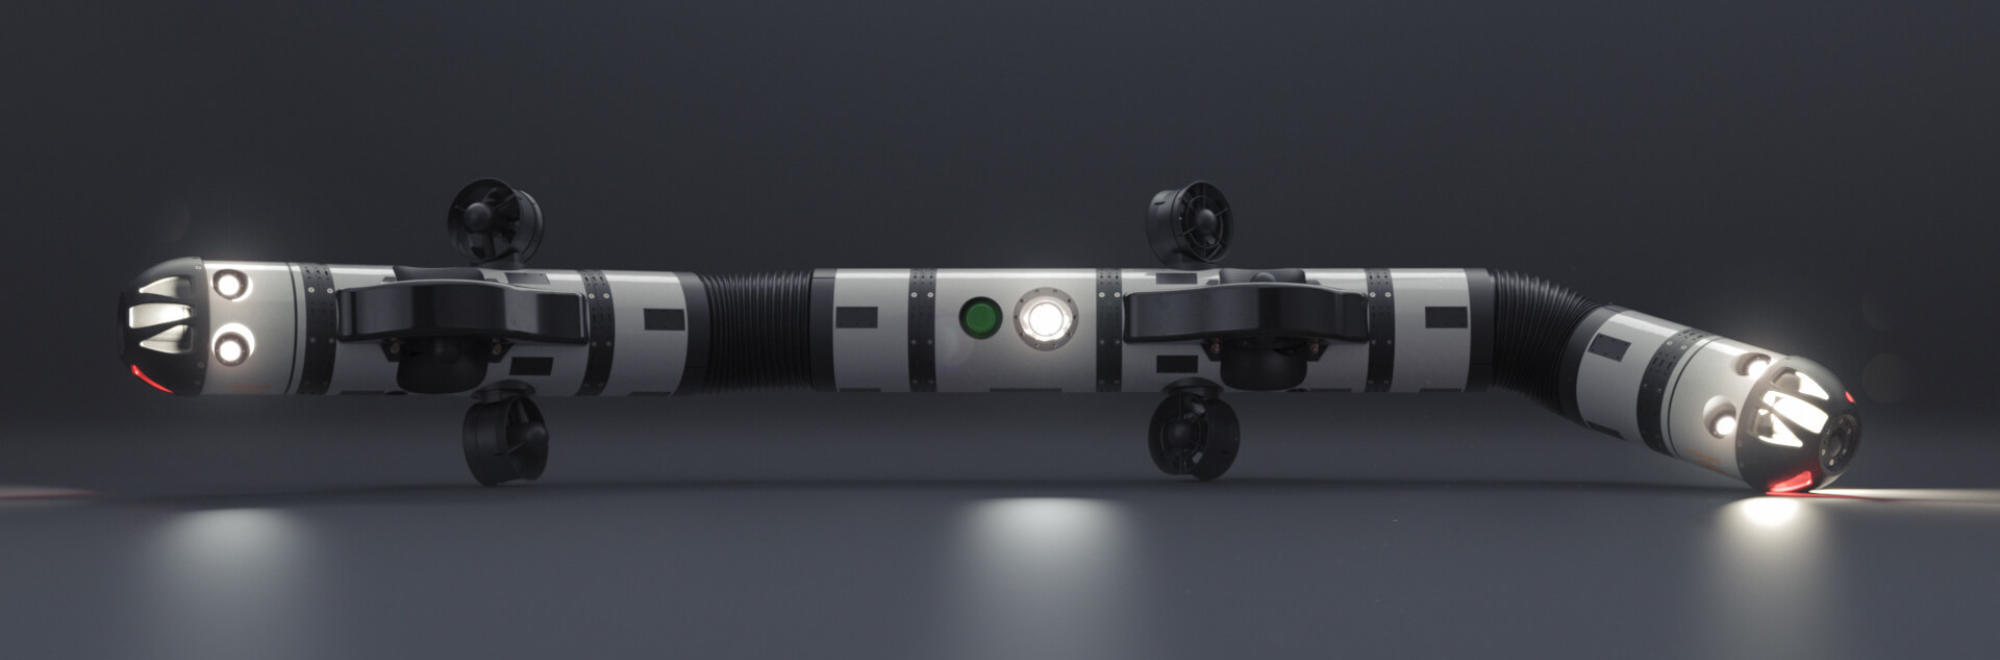
\includegraphics[width=0.8\linewidth]{assets/images/eely.jpg}
    \caption{Computer rendering of the Eelume 500 robot. Credit: Eelume.}
    \label{fig:eely}
\end{figure}

Each of the links has two degrees of freedom and is actuated by a pair of
motors. In addition, two of the links are equipped with a set of $4$ thrusters.
The thruster configuration allows the robot to move in all directions, making
the robot fully actuated. Although one can define the base of the robot as any
link, in this work, we will define the base as the middle link. The position of
the Eeelume robot is uniquely determined by the position of this base and the 
two pairs of joint angles, making the robot a 10-DOF system. The two sets of 
$4$ thrusters, as well as the two pairs of motors controlling the joints, are 
all independently actuated, making the input space of the robot a 
12-dimensional space.

We will denote each of the links with a number from $1$ to $3$, where link $1$,
the "head" of the robot, is the smallest link situated in the rightmost position
in \autoref{fig:eely}. The parameters of the Eelume robot are given in a
NED coordinate system, where the head of the robot is the most northern point.

We will assume that the robot in neutrally buoyant. In reality, weights can be
added to a module to adjust its center of mass, making the weight of the robot
equal to the weight of the water it displaces. This can however be a difficult
task as the density of water can vary, and the weights needs to be placed at 
predetermined locations meaning that one cannot place the center of mass at an
arbitrary location.
The parameters of the robot are given in \autoref{tab:robot}.

\begin{table}[h]
    \centering
    \begin{tabular}{|c|c|c|c|}
        \hline
        Parameter & Value & Unit & Description \\ \hline
        $r$ & 0.1 & m & Radius of each link \\
        $m_1$ & 40 & kg & Mass of link $1$ \\
        $m_2$ & 90 & kg & Mass of link $2$ \\
        $m_3$ & 50 & kg & Mass of link $3$ \\
        $l_1$ & 1.0 & m & Length of link $1$ \\
        $l_2$ & 2.3 & m & Length of link $2$ \\
        $l_3$ & 1.5 & m & Length of link $3$ \\
        $l_{\mathrm{joint}}$ & 0.6 & m & Length of each joint \\
        $\beta$ & 0.1 & - & Damping parameter \\
        $\gamma$ & 0.2 & - & Damping parameter \\
        $v_{\mathrm{ref}}$ & 0.1 & m/s & Reference velocity for damping \\
        $C_D$ & 0.3 & - & Damping coefficient \\
        $\rho$ & 1025 & kg/m$^3$ & Density of water \\
        \hline
    \end{tabular}
    \caption{Parameters for the simplified Eelume 500 robot.}
    \label{tab:robot}
\end{table}

The $\beta$, $\gamma$, $v_{\mathrm{ref}}$ and $C_D$ parameters specify the damping
coefficients of the robot. The damping matrix the parameters specify is given in
\autoref{eq:damping_cyl}. These parameters are based on \cite{bendik}. Added mass
is computed based on \autoref{eq:ellipsoid_added_mass}.
The inertia matrix of the robot is appriximated as a
cylinder with uniform density and is as follows:

\begin{align}
    \bm{I}_i &=
    \begin{bmatrix}
        \frac{m_i}{2} r^2 & 0 & 0 \\
        0 & \frac{m_i}{12} (3r^2 + l_i^2) & 0 \\
        0 & 0 & \frac{m_i}{12} (3r^2 + l_i^2)
    \end{bmatrix} &
    i &= 1, 2, 3.
\end{align}

The thruster configuration is similar to that of \autoref{fig:eely}. The exact
specifications of the position and orientation of the thrusters can be seen in
\autoref{tab:thrusters}.

\begin{table}[h]
    \centering
    \begin{tabular}{|c|c|c|c|c|c|}
        \hline
        Link & Thruster & $x$, North [m] & $y$, East [m] & $z$, Down [m] & Thrust Direction \\ \hline
        $2$ & Starboard & $0.56725$ & $-0.174$ & $0$ & Sout-Up \\
        $2$ & Port & $0.56725$ & $0.174$ & $0$ & Sout-Down \\
        $2$ & Bottom & $0.67725$ & $0.000$ & $0.09$ & East \\
        $2$ & Top & $0.67725$ & $0.000$ & $-0.09$ & West \\
        $3$ & Starboard & $0.02025$ & $-0.174$ & $0$ & Sout-Down \\
        $3$ & Port & $0.02025$ & $0.174$ & $0$ & Sout-Up \\
        $3$ & Bottom & $-0.08975$ & $0.000$ & $0.09$ & West \\
        $3$ & Top & $-0.08975$ & $0.000$ & $-0.09$ & East \\
        \hline
    \end{tabular}
    \caption{Thruster configuration for the simplified Eelume 500 robot. Positions relative to link center.}
    \label{tab:thrusters}
\end{table}

The transformations between the thruster positions and the link center are given
as transformations described in $\SE$. Let $\bm{T}_{\rightarrow}$ and $\bm{T}_{\angle}$
dente functions that return the transformation matrix corresponding to a translation
or rotation, respectively.
\begin{subequations}
\begin{align}
    \bm{T}_{\rightarrow} : \R^3 &\to \SE 
    &\bm{T}_{\rightarrow} :\bm{p} &= \begin{bmatrix} \I_3 & \bm{p} \\ \bm{0}_{1\times3} & 1 \end{bmatrix} \\
    \bm{T}_{\angle} : \R^3 &\to \SE
    &\bm{T}_{\angle} : \begin{bmatrix}\phi \\ \theta \\ \psi \end{bmatrix} &= \begin{bmatrix}
        \bm{R}_z(\psi) \bm{R}_y(\theta) \bm{R}_x(\phi) & \bm{0}_{3\times1} \\
            \bm{0}_{1\times3} & 1
    \end{bmatrix}.
\end{align}
\end{subequations}
The transformation matrices are then given as follows:

%Tl1_to_body = se3.trans(lengths[1]/2+jlhs, 0, 0) @ se3.rot_y(a3) @ se3.rot_z(a4) @ se3.trans(lengths[0]/2+jlhs, 0, 0)
%    Tl3_to_body = se3.inv(
%            se3.trans(lengths[2]/2+jlhs, 0, 0) @ se3.rot_y(a1) @ se3.rot_z(a2) @ se3.trans(lengths[1]/2+jlhs, 0, 0)
%            )
\begin{align}
    \bm{T}_1^2 &= \bm{T}_{\rightarrow}\left( \begin{bmatrix} \frac{l_1}{2}+\frac{l_{\textrm{joint}}}{2} \\ 0 \\ 0\end{bmatrix}\right)
        \bm{T}_{\angle}\left( \begin{bmatrix} 0 \\ a_3 \\ 0\end{bmatrix}\right)
        \bm{T}_{\angle}\left( \begin{bmatrix} 0 \\ 0 \\ a_4\end{bmatrix}\right)
            \bm{T}_{\rightarrow}\left( \begin{bmatrix} \frac{l_0}{2}+\frac{l_{\textrm{joint}}}{2} \\ 0 \\ 0\end{bmatrix}\right) \\
    \bm{T}_2^3 &= \bm{T}_{\rightarrow}\left( \begin{bmatrix} \frac{l_2}{2}+\frac{l_{\textrm{joint}}}{2} \\ 0 \\ 0\end{bmatrix}\right)
        \bm{T}_{\angle}\left( \begin{bmatrix} 0 \\ a_1 \\ 0\end{bmatrix}\right)
        \bm{T}_{\angle}\left( \begin{bmatrix} 0 \\ 0 \\ a_2\end{bmatrix}\right)
            \bm{T}_{\rightarrow}\left( \begin{bmatrix} \frac{l_1}{2}+\frac{l_{\textrm{joint}}}{2} \\ 0 \\ 0\end{bmatrix}\right) \\
    \bm{T}_2^n &= \bm{T}_{\angle}\left( \begin{bmatrix} \phi \\ \theta \\ \psi\end{bmatrix}\right)
        \bm{T}_{\rightarrow}\left( \begin{bmatrix} x^n \\ y^n \\ z^n\end{bmatrix}\right) \\
            \bm{T}_1^n &= \bm{T}_2^n \bm{T}_1^2 \\
            \bm{T}_3^n &= \bm{T}_2^n \left(\bm{T}_2^3\right)^{-1}.
\end{align}
where $a_1$, $a_2$, $a_3$ and $a_4$ are the parameters of the joint angles,
$\bm{T}_1^2$, and $\bm{T}_2^3$ are the transformations from link $1$ to link $2$
and from link $2$ to link $3$, respectively. $\phi$, $\theta$ and $\psi$ are the
Euler angles of the base and $x^n$, $y^n$ and $z^n$ are the position of base
in the NED coordinate system. Collecting the parameters describing the position
and attitude of the entire robot, we can define the state of the robot as
\begin{align}
    \bm{q} &= \begin{bmatrix} x^n & y^n & z^n & \phi & \theta & \psi & a_1 & a_2 & a_3 & a_4 \end{bmatrix}^T.
\end{align}
From the parameters stated above, the dynamics of the robot, on the form of
\autoref{eq:pymuvs:eom}, was computed using \pymuvs.

\subsection{Task Descriptions}

Two simple tasks will be used in the simulation. The first task is a position
task, where the "tail" of the robot is to be positioned at the origin of the
NED coordinate system. The second task is to drack a trajectory with the outer
most point of the "head" of the robot. The trajectory starts close to the origin,
meaning that in the beginning of the simulation, the robot will be able to
complete both tasks. As the trajectory moves further away from the origin, it
starts to rotate in the East-Down plane, making it more difficult for the robot
to complete both tasks. The trajectory eventually moves so for north that it
is impossible for the robot to complete both tasks at the same time. This
will show the prioritization of the tasks. Task $\bm{f}_1$ is the position task
and is defined as
\begin{align}
    \bm{f}_1(\bm{q}) &= \bm{T}_3^n \begin{bmatrix} -l_3/2 & 0 & 0 & 1 \end{bmatrix}^T &
        \sigma_1(t) &= \begin{bmatrix} 0 & 0 & 0 \end{bmatrix}^T,
\end{align}
where $\bm{\sigma_1}(t)$ is the desired task position. The task $\bm{f}_0$, the
trajectory tracking task, is defined as
\begin{align}
    \bm{f}_0(\bm{q}) &= \bm{T}_1^n \begin{bmatrix} l_1/2 & 0 & 0 & 1 \end{bmatrix}^T &
        \bm{\sigma}_0(t) &= \begin{bmatrix}
            0.05t + 4.33 + 0.1e^{-t} \\
            0.3 \left(1-e^{-t/8}\right)\cos{\frac{1}{2}t} \\
            0.3 \left(1-e^{-t/8}\right)\sin{\frac{1}{2}t}
        \end{bmatrix}.
\end{align}
We can see that the trajectory starts at $\begin{bmatrix} 4.33 & 0 & 0 \end{bmatrix}^T$
and moves at a speed of $0.05$ m/s in the North direction. The $0.1e^{-t}$ term
is added to make the trajectory have some non-linearities as well as
non-zero acceleration. The trajectory approaches a spiral shape as $t$ increases.

\begin{figure}[h]
    \centering
    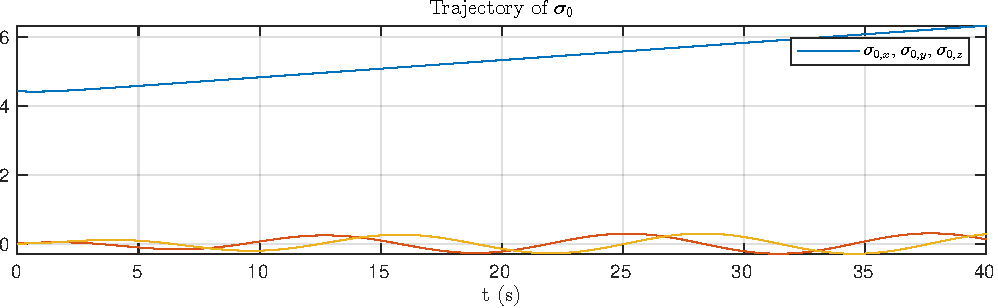
\includegraphics[width=\linewidth]{assets/plots/traj_xyz.pdf}
    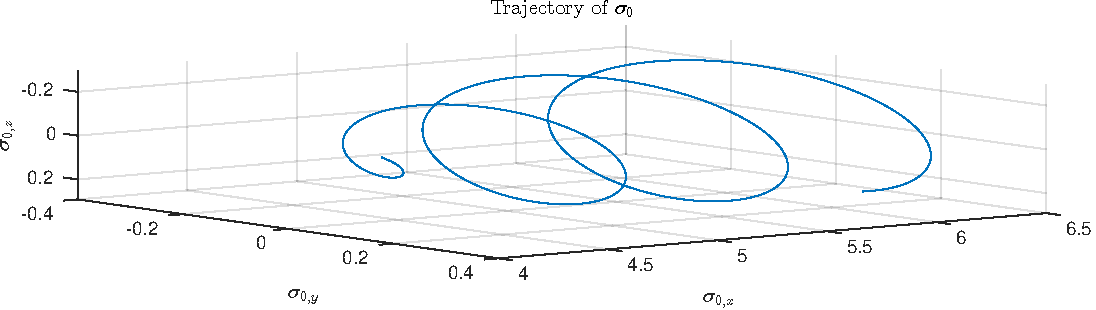
\includegraphics[width=\linewidth]{assets/plots/traj_taskspace.pdf}
    \caption{The desired task trajectory in the NED frame.}
    \label{fig:traj_f0}
\end{figure}

The task as seen in \autoref{fig:traj_f0} is the highest priority task.


\subsection{Control methods}
\subsubsection{Kinematic-level Control}

The kinematic-level control method used in the simulation is the velocity-level
controller presented in \autoref{sec:velocity_level_control}. As we are only considering
a case with two tasks, the question of successive versus augmented nullspace projections
are irrelevant. The low-levl joint-space controller chosen is a PD+ controller
with buoyancy/gravity compensation. Because of the simplicity of the shape of the robot,
these forces are relatively well known in a real-world scenario.

The gain matrices $\bm{K}_p$ and $\bm{K}_d$ as presented in \autoref{eq:Kp_Kd}
are chosen based on the assumption that the mass, coreolis, damping and added mass
matrices are known and constant. Under theis assumption, the system model is approximated
as
\begin{align}
    \bar{\bm{M}}(\bm{0}) \ddot{\bm{q}} + \bm{C}(\bm{0}, \dot{\bm{0}}) \dot{\bm{q}} +
    \bm{D}(\bm{0}, \dot{\bm{0}}) \dot{\bm{q}} + \bm{g}(\bm{q}) \approx \bm{J}^T(\bm{q}) \bm{B} \bm{u},
\end{align}
Using this approximation, the gains are chosen 

The assumptions and implications of using gains based on the model are discussed
in \autoref{sec:simulation:results}.

\subsubsection{Dynamic-level Control}

\subsection{Simulation Environment}
\begin{itemize}
    \item Mention simulator
    \item Initial conditions
    \item simulation parameters, $\Delta t$, etc.
    \item The force and torque limits of the robot.
    \item Force is pass through (no lowpass filtering), and the implications of
        this.
\end{itemize}

The initial conditions of the robot in the simulation are given in \autoref{tab:initial}.
The simulation parameters were chosen such that it satisfies task $1$, for the tail,
but not task $0$, the trajectory tracking task. This was done to show convergence
to the task when having an error in the initial conditions.
\begin{table}[h!]
    \centering
    \begin{tabular}{|c|c|c|c|c|c|c|c|c|c|c|c|}
        \hline
        Parameter & $x^n$ & $y^n$ & $z^n$ & $\phi$ & $\theta$ & $\psi$ & $a_1$ & $a_2$ & $a_3$ & $a_4$ \\ \hline
        Value & 3.17 & 0 & -1.0 & 0 & 0 & 0 & -0.59 & 0 & -0.88 & 0 \\ \hline
        Unit & m & m & m & rad & rad & rad & rad & rad & rad & rad \\
        \hline
    \end{tabular}
    \caption{Initial conditions for the Eelume 500 robot in simulation.}
    \label{tab:initial}
\end{table}

\subsection{Performance Metrics}
\begin{itemize}
    \item Task error
    \item Computation time
\end{itemize}

% -----------------------------------------------------------------------------
%\section{Simulation Scenarios}

% -----------------------------------------------------------------------------
\section{Results and Discussion}
\label{sec:simulation:results}.
\subsection{Quantitative Results}
\subsection{Qualitative Observations}
\subsection{Comparative Analysis}

\iffalse
\begin{figure}[h]
    \centering
    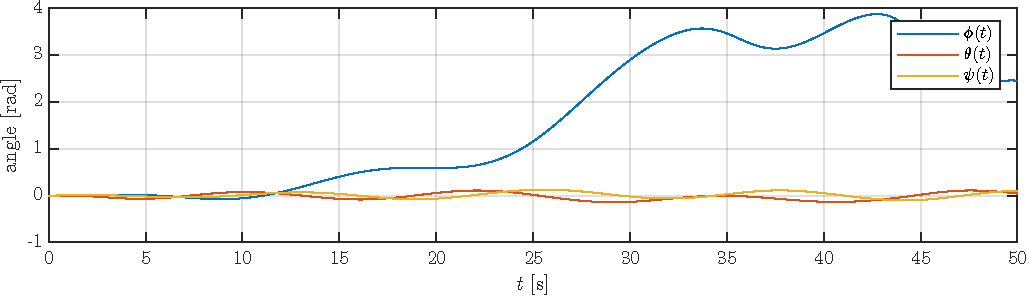
\includegraphics[page=1,width=\linewidth]{assets/plot.pdf}
    \caption{Euler angles of simulated Eelume robot with feedback linearization control.}
    \label{fig:plot}
\end{figure}

\begin{figure}[h]
    \centering
    \includegraphics[page=2,width=\linewidth]{assets/plot.pdf}
    \caption{NED position of simulated Eelume robot with feedback linearization control.}
    \label{fig:plot2}
\end{figure}

\begin{figure}[h]
    \centering
    \includegraphics[page=3,width=\linewidth]{assets/plot.pdf}
    \caption{}
    \label{fig:plot3}
\end{figure}

\begin{figure}[h]
    \centering
    \includegraphics[page=4,width=\linewidth]{assets/plot.pdf}
    \caption{}
    \label{fig:plot4}
\end{figure}
\fi

\begin{itemize}
    \item Simulation study comparing velocity- and acceleration-level task-priority
        control methods for light-UVMS.
\end{itemize}

\chapter{Conclusion and Future Work}

{\color{red}
General feedback:
\begin{itemize}
    \item Tegnsetting av alle ligninger
\end{itemize}
}


\printbibliography
\addcontentsline{toc}{chapter}{Bibliography}
\newpage
\appendix

%\chapter{Appendix}

\end{document}
